\begin{center}
    

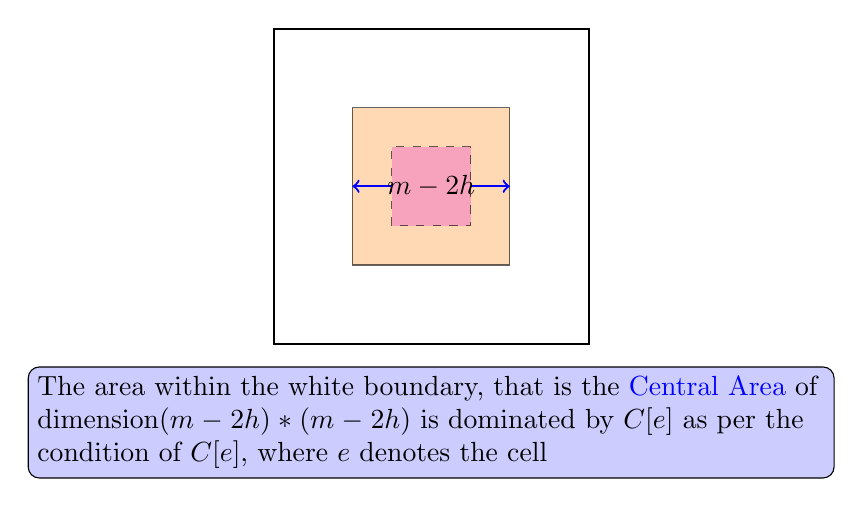
\begin{tikzpicture}

    % Square in the middle
    \draw[thick] (1, 1) rectangle ++(4, 4);
    \draw[fill=orange!50, opacity = 0.6] (2, 2) rectangle ++(2, 2);
    \draw[dashed, fill=magenta!50, opacity = 0.6] (2.5, 2.5) rectangle ++(1, 1);

    \draw[->, blue, thick ] (2.5, 3) -- (2,3) ;
    \draw[->, blue, thick ] (3.5, 3) -- (4,3) ;
    \node at (3,3) {$m -2h$};

    \node[draw, fill=blue!20, text width=10cm, rounded corners] at (3, 0) {
    The area within the white boundary, that is the \textcolor{blue}{Central Area} of dimension\textbf{$ (m-2h) * (m-2h) $} is dominated by $C[e]$ as per the condition of $C[e]$, where $e$ denotes the cell  
    };
    
     

\end{tikzpicture}

\end{center}